\documentclass[12pt, a4paper]{report}   	% use "amsart" instead of "article" for AMSLaTeX format

\usepackage{geometry}                		% See geometry.pdf to learn the layout options. There are lots.
\geometry{letterpaper}                   		% ... or a4paper or a5paper or ... 

\usepackage[parfill]{parskip}    		% To begin paragraphs with an empty line rather than an indent

%Tables
\usepackage[none]{hyphenat}  % Stops breaking up words in a table
\usepackage{array}

%Img
\usepackage{graphicx}				% To import images
\usepackage{float}						% Control of float positions

\usepackage{hyperref} % Clicable references
\hypersetup{hidelinks, urlcolor=cyan}									
\usepackage{amssymb}

\title{Mapping the  technical challenges regarding OSM, with examples from the norwegian open and free governmental data}
\author{Anne Sofie S. Erichsen}
%\date{}							% Activate to display a given date or no date

\begin{document}

%Front stuff
\pagenumbering{roman}

\maketitle

%Table of contents with no page number
\tableofcontents   
\thispagestyle{empty}
\cleardoublepage

%List of figures, list of tables
\setcounter{page}{1}
%\listoffigures
%\addcontentsline{toc}{section}{\numberline{}List of Figures}
\cleardoublepage

%\listoftables
%\addcontentsline{toc}{section}{\numberline{}List of Tables}
%\cleardoublepage

%Main document and numbering starts here
\pagenumbering{arabic}

\setcounter{page}{1}


\abstract
A big problem with OSM is finding a good, fast and easy way of correcting data. There exists multiple tools that finds possible errors, but there also has to be a good way of fixing them. A solution to this problem can be can be microtasking. Microtasks are formed basically by dividing a project into smaller tasks, clearly defined, that can be performed independently \cite{EstellesArolas}.  

\chapter{Introduction}\label{sec:intro}
This paper will inform you on the technical challenges regarding OpenStreetMap and governmental data \cite{Exel2010}. For a summary of papers you can see on page \pageref{sec:wang}

In theory micotasking seems to solve a lot of OSM problems like overlapping data, deletion of good metadata (read: tags) when running import-scripts and makes it easier to control, both the workflow and quality of the data. Microtasking splits a task into multiple subtasks and distributing these subtasks to humans over the internet.  The OSM mindset  of schema-less datasets and tags differs from many organizations. With the success of OSM it is time to start taking this mindset serious. OSM also has its weaknesses , but many people believe microtasking solves the majority of them. By using FKB building dataset I will try too look further into mapping governmental data over to the OSM format, also trying to experience if microtasking is the solution of the weaknesses of OSM, like the ones I mentioned above. 

\chapter{Characteristics of Open Street Map}

\section{General}
The OpenStreetMap project is one of the most impressive projects of Volunteered Geographic Information on the Internet\cite{Neis2012}. Until recent the mapping of the Earth was preserved highly skilled, well-equipped and organized individuals and groups. One important happening was in 2000 when Bill Clinton removed the selective availability of the GPS signal \ref{sec:weber}. This change improved the accuracy of simpler, cheaper GPS receivers so that also ordinary people could start mapping their movements. OpenStreetMap was founded in 2004 at University College London by Steve Coast. The goal was to create a free database with geographic information of the world \cite{Neis2012}. Back in 2004, the geographic data was expensive and hard to get access to. 

The OSM project stands out from other data sources mainly because it's free to use and released under a license that allows for pretty much whatever the user wants to as long as the user mention the original creator and the licence\cite{Chilton}.  The most common contribution approach is to record data using a GPS receiver and edit the data using one of the free and available OSM editors \cite{Neis2012}.  

One of the reasons for OpenStreetMap's success is that today the world has a need for instant information, particularly in crisis situations \cite{Chilton}. Here OpenStreetMap is the leading global example of the effectiveness of crowdsourcing of geodata. Crowdsourced geographic data has characteristics or advantages of large data volume, high currency, large quantity of information and low cost \cite{Wang2013}. The project is changing the way individuals and organizations are thinking about the collection process, purchase and use of geodata \cite{Chilton}.  

%\section{Culture}
%OSMhas no notability rule, an arbitrary amount of detail is possible, but somebody has to maintain it! %https://www.youtube.com/watch?v=KNTSZGnQVRw

\section{Data structure}
OpenStreetMap uses a topological data structure. This structure includes three basic components nodes, ways, and relations. Nodes are points with a geographic position stored as coordinates (Lat, long) according to WGS84. Ways are lists of two or more nodes, representing an open- or closed way used to describe streets, rivers, among others \cite{Debruyne2015}. A relation is a multi-purpose data structure that documents a relation between two or more components \cite{OpenStreetMapg}. OpenStreetMap's structure uses tags to add metadata to geographic objects. Tags consist of two items, a key and a value of the form key=value. The key is used to describe the topic, category or type of feature, while the value represents the details of the particular form of the key specified. An example of a key-value pair can be building=church, here the key is building and the value is a church, this is a building that was built as a church. 

OpenStreetMap does not have any restrictions on tags assigned to nodes, ways or relations, and mappers can use any key-value pair in their import. Nevertheless, the norm in OSM is to try to map new data with existing tags. Good practice is to search for tags, or map features, on different OSM wiki-sites. On the \textit{tags you like} wiki page they recommend different sites, but points out \textit{taginfo.openstreetmap.org} as the most useful site. Taginfo is a website created for finding and aggregating information about OSM tags, it covers the whole planet and is updated daily. The web page list tags used in the database and also inform on how often they have been used.* %How frequent they appear insted?
 Taginfo also lists other tags which have been used in combination with the displayed tag. Some countries also have their own taginfo web pages, like Ireland, Great-Britain, and France, Norway does not have it. If a mapper doesn't find an appropriate key-value pair and wants to create a new feature, this has to be documented on the OSM wiki page. 

In OSM, changes made by one user over a short period is called a changeset \cite{OpenStreetMapi}.  Change can be a creation of new components, adding tags to existing components, changes to tags in existing components, removal of tags and removal of components. Changes are added to the changeset as long as it's open, changesets are either closed directly or by itself after a period of inactivity (currently after one hour). Every component in the OSM database is a part of a changeset.* %Hvert element i OSM databasen er en del av et changeset, skrive om?

\section{Organization}
%Redgjøre for hva OSM er og hvordan det fungerer teknisk og organisatorisk
The OpenStreetMap Project is supported by the OpenStreeMap Foundation (OSMF) which is a UK-registered non-profit organization. OSMF was founded in 2006 and consists of members from all over the world, as of December 2015 consist of 350 normal-, 351 associate- and 18 corporate members \cite{OSMF2015}. OSMF include a board of seven members and is critical to the ongoing function and growth of the OpenStreetMap project \cite{OSMF}.  The foundation has the responsibility for the servers and services necessary for hosting the OSM project. They also support and communicates with the working groups, and delegates important tasks like web page development, etc. 

A person can contribute to the OSM project without being a member of the foundation. The project has over 3 million registered users, and around 40 000 active users each month \cite{ OSMstats2016} collecting, updating and editing the data. The crowdsourced data are then released under the Open Database License, \textit{"a license agreement intended to allow users to freely share, modify, and use this Database while maintaining this same freedom for others"} \cite{ODbL}.  Users can edit maps through different tools made by OSM developers. One tool is called iD and is the default web browser editor created by MapBox. There are also desktop editing applications like JOSM and Merkaartor which are more powerful and better suited for advanced users. 

Communication is done through channels like mailing lists, wiki pages, conferences and GitHub repositories. In the public mailing lists, everyone who subscribes to it is overhearing every conversation. Overhearing conversations through mailing lists is described as broadcast communication in the Gutwin paper from 2004 \cite{Gutwin2004}. The ability to speak to an expected audience rather than one individual has several advantages. Allowing people to decide for themselves whether to respond or not and as the conversation develops new people can join. In OpenStreetMap there are over 150 mailing lists \cite{Reiter2016}, keeping an overview of everything is impossible. That is why weeklyOSM was created in 2010 and is a collection of news relevant to the OSM community written in 5 different languages \cite{Freyfogle2016}.  In State of the Map 2016 conference, the WeeklyOSM team won the Influential Writing Award, nominated and voted by the community [OpenStreetMap, 2016a]. A good evidence of how important their work is to the community. State of the Map is the main OSM conference, organized by OSMF and has been held each year since 2007 \cite{OpenStreetMapj}. Important communication is also done through both issues and pull requests in the repositories at the OpenStreetMap GitHub channel. 

 \section{File format, .osm files}
The .osm file format is specific to OpenStreetMap, and it is not easy to open these files using GIS-software like QGIS. The file format is designed to be easily sent and received across the Internet in a standard format. Therefore .osm files are easily obtained, but using the files directly for analyzing and map design is not easy. The .osm files are coded in the XML format. It is recommended to convert the data into other formats when using the files \cite{Learnosm}. 

Points are represented as nodes, lines as ways and areas as a relation in .osm files. Each represented by a tag: <node>, <way> and <relation>. Node is one of the core elements in the OSM data model. A node-tag consists of a single point defined by node-id, latitude, and longitude. When nodes are used on their own, which means that they are not included in a way or a relation, they represent point features. Points features normally include at least one tag to define the points purpose \cite{OpenStreetMapc}. In listing \ref{eq:nodetag} the node tag describes a bag shop named Citybag, this is called a point of interest. The user key's value is the name of who last modified this node (user="Peter Bremer") and uid are the person's numeric user id (uid="366321"). * %Litt for tung setning?

\lstset{
    language=XML,
    morekeywords={encoding,node, tag},
    label=eq:nodetag,
    caption=Example of a node tag
}
\begin{lstlisting}
 <node id="4004323486" visible="true" version="1" changeset="37189343"
  timestamp="2016-02-13T15:58:54Z" user="Peter Bremer" uid="366321" 
  lat="63.4318129" lon="10.3971411">
  <tag k="name" v="Citybag"/>
  <tag k="shop" v="bag"/>
 </node>
\end{lstlisting}

A way-tag consists of two or more nodes and can either be open or closed. An open way describes a line feature that does not share the first and last node. Examples of features are roads, cycleway, and streams. When a way is closed the first and last nodes are the same and can be interpreted as a closed polyline or an area, or both \cite{OpenStreetMapd}. A closed way with highway=* tag can represent roundabouts, or if it has amenity=school tag the closed way represent the outline of a school. In listing \ref{eq:waytag1} the way describes a building outline since the key equals building and the value equals church.  The building in listing \ref{eq:waytag1} is the footprint of a church. The <nd> tag represents a node, where the <nd> tags refers to <node> tags who contains the lat, long values. All <nd> tags create the building footprint, notice that there is no height parameter. Listing \ref{eq:waytag1} creates a 2D representation of the church which is shown in figure \ref{fig:fruekirke2D}. A 3D representation of the same church is shown in figure \ref{fig:fruekirke}.

\lstset{
    language=XML,
    morekeywords={encoding, relation, way, tag, node, member},
    label=eq:waytag1,
    caption=Example of a way tag - creating the building footprint of a church
}
\begin{lstlisting}
 <way id="89340594" visible="true" version="6" changeset="42571811" 
  timestamp="2016-10-01T22:11:17Z" user="Peter Bremer" uid="366321">
  <nd ref="1036369169"/>
  <nd ref="1036369134"/>
  <nd ref="1036369111"/>
  <nd ref="1036369185"/>
  <nd ref="1036369163"/>
  <nd ref="1036369118"/>
  <nd ref="1036369099"/>
  <nd ref="4427055078"/>
  <nd ref="1036369179"/>
  <nd ref="1036369158"/>
  <nd ref="4427055082"/>
  <nd ref="1036369145"/>
  <nd ref="1036369124"/>
  <nd ref="1036369103"/>
  <nd ref="4215548739"/>
  <nd ref="4215548736"/>
  <nd ref="4215548737"/>
  <nd ref="4215548740"/>
  <nd ref="1036369182"/>
  <nd ref="1036369140"/>
  <nd ref="1036369115"/>
  <nd ref="1036369096"/>
  <nd ref="1036369135"/>
  <nd ref="1036369149"/>
  <nd ref="4427055803"/>
  <nd ref="1036369131"/>
  <nd ref="1036369107"/>
  <nd ref="1036369169"/>
  <tag k="amenity" v="place_of_worship"/>
  <tag k="building" v="church"/>
  <tag k="denomination" v="protestant"/>
  <tag k="name" v="Vår Frue kirke"/>
  <tag k="religion" v="christian"/>
  <tag k="wheelchair" v="yes"/>
  <tag k="wikidata" v="Q3356455"/>
  <tag k="wikipedia" v="en:Vår Frue Church"/>
 </way>
\end{lstlisting}

\begin{figure}[H]
    \centering
    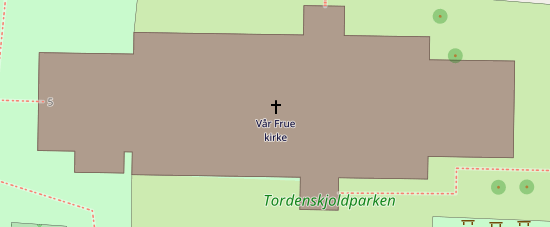
\includegraphics[scale=0.5]{figures/FixedByMe/fruekirke2D.png}
    \caption{2D representation of \textit{Vaar frues kirke}, result of listing \ref{eq:waytag1}. Source: openstreetmap.org}
    \label{fig:fruekirke2D}
\end{figure}

A relation is an ordered list of one or more nodes, ways, and/or relations and is used to define logical or geographical relationships between the other elements \cite{OpenStreetMape}. If a building consists of multiple parts, tagged with building:part=*, a relation is used to define the geographical relationship between the parts. Specifying roles to different parts is possible. A road can have role as east, going towards east. In multi-polygons, parts can have an inner or outer role, to specify whether it forms the inner or outer part of the polygon. A building relation is shown in listing \ref{eq:reltag}. There are eight members in this relation. The first member is a way, and it has an outline role creating the building footprint, for 2D representation. Listing \ref{eq:waytag1} is the XML-code for this way (notice that the ref number are equal to the way id in listing \ref{eq:waytag1}). The only node member in the relation contains the church's address. The rest of the members creates the 3D representation of the building shown in figure \ref{fig:fruekirke}.

\lstset{
    language=XML,
    morekeywords={encoding, relation, way, tag, node, member},
    label=eq:reltag,
    caption=Example of a relation tag - creating 3D representation of a church
}
\begin{lstlisting}
 <relation id="6269954" visible="true" version="2" changeset="39708156" 
  timestamp="2016-06-01T11:14:18Z" user="Peter Bremer" uid="366321">
  <member type="way" ref="89340594" role="outline"/>
  <member type="node" ref="2957446972" role=""/>
  <member type="way" ref="421821942" role=""/>
  <member type="way" ref="421821938" role=""/>
  <member type="way" ref="421821939" role=""/>
  <member type="way" ref="421821940" role=""/>
  <member type="way" ref="421821937" role=""/>
  <member type="way" ref="421821941" role=""/>
  <tag k="name" v="Vår Frue kirke"/>
  <tag k="type" v="building"/>
 </relation>
\end{lstlisting}

\begin{figure}[H]
    \centering
    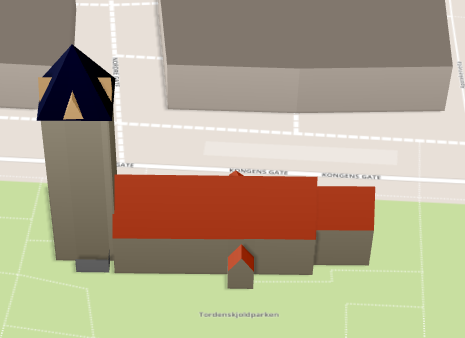
\includegraphics[scale=0.5]{figures/FixedByMe/fruekirke.png}
    \caption{3D representation of \textit{Vaar frues kirke}, result of listing \ref{eq:reltag}. Source: osmbuildings.org}
    \label{fig:fruekirke}
\end{figure}


 \section{Mapping buildings in OSM}\label{buildOSM}
A building can be represented by nodes, ways or relations in OpenStreetMap. When importing buildings into OSM, the XML-code representing the building must be tagged with Building=*. Frequent occurring values are house, residential and garage, describing the buildings particular usage.  Using the building tag in node representations is tolerated but not recommended. A building is much better expressed by their footprint (close way or multi-polygon), and if the footprint is available, one should not add the building key in nodes. The building key should be used to mark the buildings footprint. The most common occurring value for the building key is yes and used when it's not possible to determine a more accurate value \cite{OpenStreetMapf}. A list of possible values that can be added to the building key is listed on the OSM building wiki page. It is possible to introduce new values, but it is not recommended. The building key is most common used in way representations \cite{TagInfo2016}. An example of how to use building key in a way-tag see listing \ref{eq:waytag1}.

A building can also be represented by a relation. Relations are used if the building consists of multiple parts which physical differ from each other, often when a 3D representation of the building is created. A building relation mainly consists of two or more ways. A way then represents a part of the building and should be tagged with a building:part key and usually the value yes. Then the way-tags representing the different building parts are ordered together inside the relation. An example of a building:part=yes implementation can be seen in listing \ref{eq:waytag}. Note that the first and last <nd> tag refers to the same node, so this is a closed way. The key roof:shape with value gable gives the appearance of the roof. The result from the code in listing \ref{eq:waytag} is shown in figure \ref{fig:erkeinng} marked with a red line. A relation containing building:parts are shown in listing \ref{eq:reltag}. Notice that this relation is tagged with the key type and the value building. If a relation is tagged with type=building, it groups both building footprint and all building parts together. See figure \ref{fig:fruekirke} for a 3D building representation created with building parts. 

\lstset{
    language=XML,
    morekeywords={encoding,way, tag, nd},
    label=eq:waytag,
    caption=Example of a way tag - creating 3D representation of a building part
}
\begin{lstlisting}
  <way id="17533469" visible="true" version="22" changeset="39301425" 
  timestamp="2016-05-13T21:20:04Z" user="Peter Bremer" uid="366321">
  <nd ref="3505716655"/>
  <nd ref="2517225923"/>
  <nd ref="4184346715"/>
  <nd ref="3505716656"/>
  <nd ref="4184346713"/>
  <nd ref="4184346717"/>
  <nd ref="3505716654"/>
  <nd ref="4184346719"/>
  <nd ref="3505716655"/>
  <tag k="building:colour" v="#c3c0b9"/>
  <tag k="building:material" v="stone"/>
  <tag k="building:part" v="yes"/>
  <tag k="height" v="11"/>
  <tag k="name" v="Sydkapell"/>
  <tag k="roof:height" v="4"/>
  <tag k="roof:material" v="copper"/>
  <tag k="roof:orientation" v="across"/>
  <tag k="roof:shape" v="gabled"/>
 </way>
\end{lstlisting}

\begin{figure}[H]
    \centering
    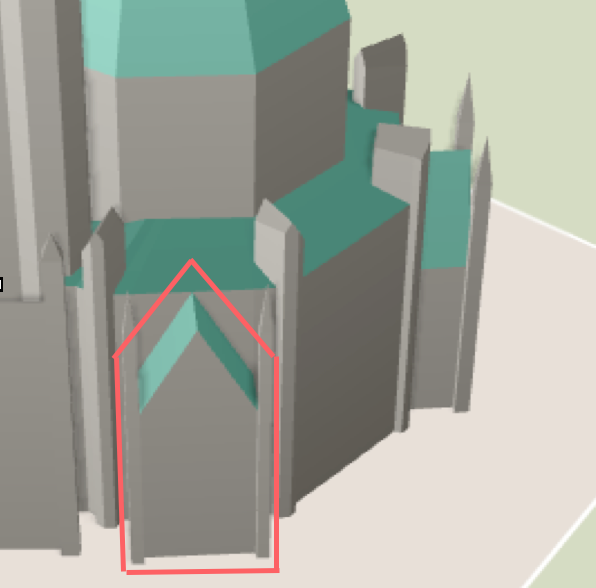
\includegraphics[scale=0.5]{figures/FixedByMe/nidaros3D.png}
    \caption{\textit{Sydkapell} with gabled shaped roof, result of listing \ref{eq:waytag}. \textit{Source: osmbuildings.org}}
    \label{fig:erkeinng}
\end{figure} 

\chapter{Technical}

\subsection{Existing libraries}
The internet consists of hundreds of software libraries and packages. It can be overwhelming for newcomers and hard to find the most suited ones. A good tip is to learn the handful of libraries and packages that most software is derived from, so called root libraries. They are actively maintained and not significantly derived from any other libraries. The libraries do geospatial operations that are hard to implement, so people choose to use the libraries instead. Geospatial datasets are large, often complex and varied. This makes the implementation harder, and some of the reasons for the libraries success. The root libraries are GDAL, OGR, GEOS and PROJ. 4 \cite{Lawhead2013}.  They are, according to J. Lawhead, "the heart and soul of of the geospatial analysis community". All the libraries are written in C or C++. 





\chapter{OSM import methods}
%1. Helautomatisk, scriptet import \\
%2. Helmanuell import basert p� tracing av f.eks WMS-data\\
%3. Guidet automatisk import (slik import av n50-data blir gjort i OSM i dag) \\
%4. Import basert p� metodikken LA-buildings-prosjektet har gjort, og som beskrives av McAndrews (microtasking)

%Conflation \href{http://wiki.openstreetmap.org/wiki/Conflation}{Wiki Conflation}
\subsection{Introduction}
The traditional way to contribute data to the OpenStreetMap project is through active users who use their GPS to track roads and their local knowledge to add information about their geographic regions to the OSM database \cite{Zielstra2013}. Users also digitalize aerial photos. Cheaper GPS receivers and more available satellite imagery with better resolution makes it easier for users to contribute \cite{Chilton}. The number of active users in different regions varies a lot, making some areas on the OSM map full of data while others are almost empty. This led to a second approach for getting data in to the OpenStreetMap database, bulk imports \cite{Zielstra2013}.  Bulk imports is the process of uploading external data and were meant for initial/preliminary object class uploads, so only if the object were none existing in the area  \cite{Zielstra2013}.  Its a good alternative for countries or regions with less active users. Through the years different import methods has been developed. This paper will evaluate the most common methods. 

\subsection{Fully automatic import script}
Creating a script that automatically imports big datasets into OpenStreetMap, a bulk import, is not encouraged in the OSM community \cite{Zielstra2013}. This becomes clear when reading the wikipages about import. A bulk import is suppose to be a supplement to user generated data. The user generated data and the users ability to work is always the priority \cite{OSMimport}. Automatic edits is changes that has no or very limited human oversight \cite{OSMAutiEdit}. This kind of edits must follow the Automated Edits code of conduct \cite{OSMAutomaticEdits}. A fully automatic import do automated edits to the OpenStreetMap database with little, if any, verification from a human. 

An example of a bulk import was the TIGER import. The Topologically Integrated Geographical Encoding and Reference system (TIGER) data was produced by the US Census Bureau and is a public domain data source. The bulk import was completed in early 2008 \cite{Zielstra2013}, populating the nearly empty map of the United States. The TIGER data was not perfect and had it's faults, but it was better than no data at all \cite{Willis2008}. 

On the TIGER OpenStreetMap wikipage, last updated August 2016, they say it is unlikely that the TIGER data ever will be imported again. The main reason is the growing US mapping community, their mapping is often better than the TIGER data. "Do not worry about getting your work overwritten by new TIGER data. Go map!" \cite{WikiOSMTIGER2007}. A new bulk import with updated TIGER data can overwrite existing, more precise data. The TIGER data are of variable quality, poor road alignment is a huge problem and also wrong highway classification. Many hours of volunteer work could be lost and this is something the community want to avoid. The bulk import in 2007 got the United States on the OSM-Map and saved the mapping community a lot of time finding road names etc. "TIGER is a skeleton on which we can build some much better maps" \cite{Willis2007}. On the negative side the project kept the US mappers away, they were told for years that their work was no longer needed after the TIGER upload was complete. But the presence of TIGER data ended up not eliminating the need for volunteer help, they needed help fixing errors like the poor road alignments. 

Bulk imports are overall not recommended today, but have been helpful as well. In the Netherlands bulk imports have meet little resistance, mainly because the imports are done by dedicated OpenStreetMap mappers who knew the OSM import guidelines.  Arguments in favor of bulk imports say that a map that already contains some information is easier to work on and can help lower the entry barriers for new contributors. Another argument is that a almost complete map is more attractive for potential users, that again can encourage more use of OSM data in professional terms \cite{Exelvan2010}. But a huge minus to bulk imports are the data aging, since the data being imported often already is a few years old and updating it takes time, often years. The TIGER import was data from 2005, but the import finished in 2007 \cite{Zielstra2013}. Between the time of first import and update the community have fixed bugs, added important metadata, the community would not want to loose that data/information. 

Today there are huge amounts of object types in OpenStreetMap. Often bulk import overrides existing data which is one of the "don't do" points on the import guidelines list on the osm wiki page. OpenStreetMap do not have layers, so data on top of data makes it very difficult to organize and find the data.   
%has common errors like wrong road classifications, adds roads that no longer or never existed, railway and roads 
%moved so they intersect when they do not. 

\subsection{Fully manually import, user generated content}
This method can be very time consuming. The mapping quality depends on the image resolution in the area beeing mapped, it is also hard to add metadata from a image. For instance, its impossible to see the height of a building from a satellite image. 

Haiti project, and other Humanitarian OSM project, draw from satellite image dry. A huge problem with this is when during a crisis, many users map the same areas. During Haiti project a problem was overlapping data, the same road drawn multiple times. This was before tasking manager. 

This method is also used today. Humanitarian OSM use the method with the tasking manager. Then the problem with overlapping data are not as likely to occur.  This import method do not require any mapping skills

	- User Generated Content providers / crowdsourced data collectors are allowed to collect geodata
		? Reason: More available satellite imagery, cheaper GPS units, etc
OSM the leading global example %CROWDSOURCING IS RADICALLY CHANGING THE GEODATA LANDSCAPE: CASE STUDY OF OPENSTREETMAP 



\subsection{Guided automatic import}\label{guidedautoimp}
Fully automatic import of huge amounts of data is discouraged in the OSM community, so another approach is guided automatic import. The OSM community encourages people to import only small amounts of data at a time and only after validation and correcting errors \cite{Mehus2014}. This method was used when the OSM-community in Norway got approval from the Norwegian map authority to import N50 data \cite{Kihle2014}. N50 is the official topographic map of Norway. The import process is described on the OSM wikipage. It says that they will import one municipality at a time. Each municipality dataset will be divided up in a .15 deg times .15 deg grid changeset and imported grid by grid* \cite{OSMN502014}. The N50 import was an community import, but only experienced user were encouraged to import the data \cite{Mehus2014}. 

The norwegian OSM group started importing the N50 data before they had consultet with the OSM imports mailing list, which is required. This was pointed out by DWG member Paul Norman \cite{Mehus2014}.  DWG is the data working group and they are authorized by the OSMF to detect and stop imports that are against the import guidelines \cite{OSMDWG}. 

Sosi to osm


\subsection{Import based on LA-buildings methodology}

OSM Tasking Manager was created in the aftermath of the Haiti earthquake. This innovation coincided with the growing popularity of microtasking as a solution to manage distributed work %Success & Scale in a Data-Producing Organization og Palen, L., Soden, R., Anderson, T. J., & Barrenechea, M. (2015). Success & Scale in a Data-Producing Organization. Proceedings of the 33rd Annual ACM Conference on Human Factors in Computing Systems - CHI ?15, 4113?4122. http://doi.org/10.1145/2702123.2702294.

The Guided automatic import from \ref{guidedautoimp} we saw that dividing datasets into smaller parts makes the import easier to, among others, distribute the workload between experienced users. OSM Tasking manager takes this approach further so that users can work on the same time with nearby areas. The tasking manager divides the areas into grids and use colors to inform the user if the grid is done, locks it if someone is already working in the grid and also the user easily can see the commit story when they click a grid. 

% LA building cleanup https://lists.openstreetmap.org/pipermail/imports/2016-August/004557.html
%Building import Oct 2016 https://lists.openstreetmap.org/pipermail/imports/2016-October/thread.html 
%This is the import OSM mailinglist 

 

%Chapter: FKB
%  About SOSI
%	 Data quality, how is the data produced
%	 Metadata - SOSI
%  Metadata - OSM, how is Trondheim covered today?
% 3D buildings Mapbox, how is the logic similair with SOSI?  https://www.mapbox.com/blog/mapbox-studio-building-heights/
% 3D modeling OSM
	%http://wiki.openstreetmap.org/wiki/Roof_3D_modeling
	%http://wiki.openstreetmap.org/wiki/3D_modeling
	%http://wiki.openstreetmap.org/wiki/Simple_3D_buildings
	%http://forum.openstreetmap.org/viewtopic.php?id=32131
% Licence, not public yet

\chapter{Summary of papers}

\subsection{Quality analysis of open street map data \cite{Wang2013}}\label{sec:wang}
Crowd sourcing geographic data is an opensource geographic data which is contributed by lots of non-professionals and provided to the public. Compared with conventional data collection and update methods, the crowd sourced geographic data has characteristics or advantages of large data volume, high currency, abundance information and low cost and becomes a research hotspot of international geographic information science in the recent years.\\ 
The primary problem is to analyse the quality of crowd sourcing geographic data. 
There are three factors that influence the quality of OSM: First data collected and mapped by non-professionals, secondly the collected data may be from different data sourcing with different precision and thirdly the data collected by different GPS may have different precisions. \\
The paper assesses three quality elements: 1. Data completeness, 2. Attribute accuracy and 3. Position accuracy. 

Enter twice to get spacing between paragraphs.

\paragraph{Data completeness}
Includes length completeness and name completeness. Length completeness is the geometric quality and data coverage. Formula: $Q_{L}=\frac{L_{OSM}}{L_{R}}$ \\(L = percentage of the length).  
\paragraph{Name completeness}
Name completeness means the completeness of the name attribute. 

\subsection{User generated Street Maps \cite{Weber2008}}\label{sec:weber}
Until recently the mapping of the Earth was preserved highly skilled, well-equipped and organized individuals and groups. The big change happened in 2000 when Bill Clinton removed the selective availability of the GPS signal, this provided much improved accuracy for simple, low-cost GPS receivers. The wide availability of high-quality location information has enabled mass-market mapping based on affordable GPS receivers, home-computers and the Internet. 
\paragraph{OSM background}
OSM follows the peer production model that created Wikipedia. Its aim is to create a set of map data thats free to use, editable, and licensed under new copyright schemes. Was founded in 2004 at University College London. In May 2008 OSM had more than 33,000 registered users and about 3,500 currently active contributors. OSM decided to follow the route of allowing only registered users to edit the map, this way they can trace the information source. OSM GeoStack is the set of tools that lets users capture, procedure, communicate, aggregate, and consume the geographical information produced in the project.  
\paragraph{Editing Tools}
OSM developers implement tools to facilitate user contributions to the database. In 2008 they had a Flash-based editor called Potlatch. Today JOSM is more common, even though this is used by more experienced OSM contributors. At the end of 2006, Yahoo granted OSM the right to use its satellite imagery to trace roads and other features. 

\subsection{\href{http://icaci.org/files/documents/ICC_proceedings/ICC2009/html/nonref/22_6.pdf}{CROWDSOURCING IS RADICALLY CHANGING THE GEODATA LANDSCAPE: CASE STUDY OF OPENSTREETMAP \cite{Chilton}}}\label{crowdsourcing}
Examining the effect of the changing cartography has on data collection using OSM crowdsourcing as a case study. Are parallels to what is happening with data collection in other aspects, like WIKIPEDIA, Flickr and YouTube. \\

	- Today: A need for instant information, particularly in crisis situations\\
	- User Generated Content providers / crowdsourced data collectors are allowed to collect geodata\\
		- Reason: More available satellite imagery, cheaper GPS units, etc \\
		- OSM the leading global example \\
		- OSM was the first online mapping service to accurately map and display the new London Heathrow Terminal 5, on the official opening day. \\
	- OSM project \href{http://wiki.openstreetmap.org/wiki/No:Main_Page} - the achieved coverage, its accuracy, availability and global impact are all changing the way individuals and org are thinking about the collection, purchase and use of geodata. \\
	- Makes OSM stand out from other data sources: \\
		- Completely free of charge \\
		- Is released under a license which allows you to do pretty much what you like \\
			As long as you mention the original creator and the license 
			\href{http://wiki.openstreetmap.org/wiki/OpenStreetMap_License} \\
	- The availability, accuracy and price of OSM data has lead some local authorities in the UK to question the need to have total reliance on being locked into a contract for their geodata with the National Mapping Agency. \\
	- OSM gives the possibility of having really current data available, other services may have a large lead for getting the data from survey to map output. \\
OSM have specialist maps for cycling, routing, applications, skiing, topography and for maritime use. 

\subsection{\href{http://www.giscience2010.org/pdfs/paper_213.pdf}{The impact of crowdsourcing on spatial data quality indicators}}
Introduce the concept "Crowd Quality" (CQ) to describe and quantify the quality of crowdsourced geospatial information. Together with the growth in volume, the usage of crowdsourced geospatial info. grew extensively as well.

	- Quality: Has a meaning if we have a common understanding of its definition \\
		 - ISO19113(2002): Quality is the "totality of characteristics of a product that bear on its ability to satisfy stated and implied needs".  \\
	 - Van Oort: Identified eleven elements of spatial data quality. The elements are used to describe the quality of geo-data collected and produced. \\
	  -  Uniform method to produce and process the data --> Homogenous and consistent quality \\
	- Crowd Quality (CQ): \\
		- 2 dim.: \\
			1. User-related quality aspects: Quality of information from an individual contributors perspective. This is the typical char. of crowdsourced data.\\
			2. Feature-related quality aspects: Perspective of the spatial feature. \\
			
	1. 3 components: Local Knowledge, Experience and Recognition. \\
		a. Familiarity to an area can be correlated to the quality of the users contribution \\
		b. Quality of a users contribution is correlated with his overall experience in contributing to the project \\
		c. Online social networks that allow for user contributions, often feedback are established (ratings, recognition for specific contributions). This type of User recognition is largely unknown in crowdsourced geospatial data --> Puts a strain in our ability to assess CQ. \\
	2. In crowdsources datasets quality elements can be different for similar features, one user can add his personal attributes when adding a restaurant in OSM, while another restaurant only have one attribute. In traditional datasets the quality elements will be uniform, have the same attributes. \\ 
		a. Quality elements that are particular interesting, since they are not consistent for crowdsourced data: \\
			1. Lineage, positional accuracy and sematic accuracy.  \\
			When data is imported from other sources, these imported features have a very clear lineage with regard to positional accuracy and precision. When imported from GPS data, the positional accuracy is harder to establish. \\
Sematic accuracy  - related to the completeness and internal consistency of the attribute metadata. A schema for attribute metadata is not common in crowdsources geospatial data projects --> Create a threat to internal consistency. 

\chapter{Movies}
\subsection{\href{http://stateofthemap.us/2015/less-bots-more-humans-using-maproulette-to-import-data/}{State of the Map, microtasking}}\label{sec:movie}
A bot is a tool that carries out repetitive and mundane (dagligdagse) automated edits on a regular basis to help maintain OSM. Most bots deal with tagging, ex xybot. BugBuster deals with removing nodes. Czechreg deals with changing geometries. 

Issues with importing: The person need to have experience with the tool and the data, but also need to have the time to manually verify each task. Therefore we have microtasking - A process of splitting a task into multiple subtasks and distributing these subtasks to humans over the internet. He things this is the way of the future. Breaking up tasks tools - OSMLY, MapRoulette, BattleGrid. They can solve our issue, but we need different tools. One to determine conflicting objects,  saving the tasks in a backend and then make a usable and easy frontend to work on the tools. \href{http://wiki.openstreetmap.org/wiki/OSM_Tasking_Manager}{OSM Tasking manager, divide up a mapping job}.

Microtasked conflation may lead to standard procedures that can help other groups import data.  Can help provide a validation step to force someone to look at each and every contribution. 


\bibliography{prosjektoppg.bib}
\bibliographystyle{apalike}
\end{document}  